
% Options for packages loaded elsewhere
\PassOptionsToPackage{unicode}{hyperref}
\PassOptionsToPackage{hyphens}{url}

\documentclass{article}
\usepackage[a4paper,
    left=2cm,
    right=2cm,
    top=2.5cm,
    bottom=2.5cm
]{geometry}

\usepackage{amsmath,amssymb}
\usepackage{graphicx}
\graphicspath{{figures/}{figures/latex-figures/}}

\usepackage{iftex}
\ifPDFTeX
  \usepackage[T1]{fontenc}
  \usepackage[utf8]{inputenc}
  \usepackage{textcomp}
\else
  \usepackage{unicode-math}
  \defaultfontfeatures{Scale=MatchLowercase}
  \defaultfontfeatures[\rmfamily]{Ligatures=TeX,Scale=1}
\fi

\usepackage{lmodern}
\usepackage{upquote}
\usepackage{microtype}
\usepackage{bookmark}
\usepackage{xcolor}
\usepackage{longtable,booktabs,array}
\usepackage{calc}
\usepackage{caption}
\usepackage{float}
\captionsetup{justification=centering}
\usepackage{etoolbox}

\makeatletter
\@ifundefined{KOMAClassName}{
  \IfFileExists{parskip.sty}{
    \usepackage{parskip}
  }{
    \setlength{\parindent}{0pt}
    \setlength{\parskip}{6pt plus 2pt minus 1pt}
  }
}{
  \KOMAoptions{parskip=half}
}
\makeatother

\setlength{\emergencystretch}{3em}

\providecommand{\tightlist}{
  \setlength{\itemsep}{0pt}
  \setlength{\parskip}{0pt}
}

\setcounter{secnumdepth}{5}

\IfFileExists{xurl.sty}{\usepackage{xurl}}{}
\urlstyle{same}

\hypersetup{
  pdftitle={Phase 1 Technical Report},
  pdfauthor={Maria SAADI, Cerine BENMEDGHAR, Sarah GHERBI, Nour El Houda AKHDARI},
  hidelinks,
  pdfcreator={LaTeX via pandoc}
}

\begin{document}

% ================= TITLE PAGE =================

\begin{titlepage}
    \centering
    \hypersetup{pageanchor=false}

    \vspace{1cm}

    {\Large University of Algiers 1}\\[0.3cm]
    {\large Faculty of Sciences}\\[0.3cm]
    {\large Department of Computer Science}

    \vspace{2cm}

    {\Huge\bfseries A Comparative Study of RAG Techniques for Generating Image Captions}

    \vspace{0.8cm}

    {\Large Phase 1 Technical Report}

\vfill

{\large\textbf{Presented by:}}\\[0.5cm]

Cerine BENMEDGHAR\\
Nour El Houda AKHDARI\\
Sarah GHERBI\\
Maria SAADI\\
    

    

\end{titlepage}
\hypersetup{pageanchor=true}
\pagenumbering{arabic}
\setcounter{page}{1}

% ================= TABLE OF CONTENTS =================

\tableofcontents

\newpage

% ================= REPORT CONTENT =================

\section*{Phase 1 Technical Report}
\label{phase-1-technical-report}

\subsection*{A Comparative Study of RAG Techniques for Generating Image Captions}
\label{a-comparative-study-of-rag-techniques-for-generating-image-captions}

\subsection*{Abstract}

% Continue your existing abstract and report here.


Automatic image captioning is an important task in computer vision and natural language processing. However, vision-language models may omit objects, describe objects that are not present, or fail to accurately represent visual attributes and relationships. Retrieval-Augmented Generation (RAG) offers a potential solution by providing relevant visual and textual information to support caption generation.

This project aims to investigate how different RAG techniques influence the quality, relevance, and visual grounding of generated image captions using the MS COCO 2017 dataset. The main motivation is to determine whether incorporating retrieved evidence can improve caption accuracy, reduce hallucinations, and provide a better balance between generation quality and computational cost.

The first phase focuses on building a reproducible data preparation and retrieval framework. It includes a knowledge base of 10,000 images and 50,000 captions, alongside a 100-image validation set and a separate 100-image legacy test set; the official evaluation uses 1,000 images. The pipeline covers image and caption preprocessing, metadata extraction, embedding generation, FAISS indexing, exploratory data analysis, and anti-leakage validation. Five retrieval configurations based on CLIP, SigLIP, and DINOv2 were evaluated using CIDEr scores on the validation set. SigLIP image-to-text achieved the highest validation CIDEr score of 0.7223 and was selected as the best-performing configuration.

At this stage, the evaluation focuses on retrieval performance rather than generated captions.

\textbf{Keywords:} MS COCO, image captioning, retrieval-augmented
generation, CLIP, DINOv2, SigLIP, Sentence-BERT, FAISS, data leakage.



\newpage

\setcounter{section}{0}
\section{Introduction and Problem
Statement}\label{introduction-and-problem-statement}

The objective of this project is to study retrieval-based methods for
generating image captions. Image caption generation normally requires an
image encoder, a language-generation model, and an image-text interface;
in a retrieval-augmented formulation, the system first retrieves
relevant images or captions from an external knowledge base and then
uses that evidence as conditioning context. Phase 1 is a
data-engineering and benchmarking phase rather than an implementation of
the final caption generator. It therefore prepares a common, verified
corpus and the retrieval infrastructure that later groups can use
consistently.

Phase 1 builds a clean, shared image-caption dataset, prevents data leakage, selects the best encoder using validation data, and establishes a retrieval baseline that finds similar images or captions without generating new captions.

The scientific deliverable is not a claim that Phase 1 itself generates
captions. Instead, it supplies a retrieval baseline using
nearest-neighbour candidates and compares candidate captions with
reference captions. This distinction is reflected in the experimental
vocabulary: an image-to-image configuration retrieves KB images and then
uses an associated caption, while an image-to-text configuration
retrieves a KB caption vector directly. Both can serve as precursor
evidence for later retrieval-augmented generation.


\section{Dataset Description}\label{dataset-description}

The project uses MS COCO 2017 \cite{fleet_microsoft_2014}. COCO provides images with object-instance
annotations and five or more human-authored captions associated with
many images. This report is restricted to the implemented Phase 1
sizes documented in Table~\ref{tab:release-composition}. The
KB contains 10,000 images and 50,000 retained captions, whereas
validation and test each contain 100 images and 500 raw
reference-caption rows. The project specification is inconsistent about the
test size (100 images in sections 4.1/4.2, 1,000 in section 4.4); the
instructor indicated verbally that the test set must contain 1,000 images
(no written confirmation is on record). The official evaluation set is
therefore a 1,000-image COCO val2017 sample (Section~\ref{official-test-results}),
and the 100-image test of release g1-v1.1 is kept unchanged as a legacy set.
In Sections 2--11.1, ``test'' denotes this legacy 100-image test unless stated otherwise.

\begin{table}[H]
\centering
\caption{Release composition (frozen release g1-v1.1; the official 1,000-image test is described in Section~\ref{official-test-results}).}
\label{tab:release-composition}
\begin{tabular}{llrr}
\toprule
Split & Source & Images & Captions/references \\
\midrule
Knowledge base & COCO train2017 & 10,000 & 50,000 KB captions \\
Validation & COCO train2017 & 100 & 500 references \\
Test & COCO val2017 & 100 & 500 references \\
\midrule
\textbf{Total} & & \textbf{10,200} & \textbf{51,000} \\
\bottomrule
\end{tabular}
\end{table}

Table 1 summarizes the dataset composition. The KB and validation
sets come from separate selections of COCO train2017, while the test
set comes from COCO val2017.

Duplicate removal is important because repeated images can cause data
leakage, bias evaluation results, and reduce retrieval diversity.
It also avoids unnecessary storage and embedding computation.
This is particularly important for SigLIP and FAISS, where duplicate
images could occupy multiple positions in the retrieval results.


\section{Dataset Splitting and
Stratification}\label{dataset-splitting-and-stratification}

\subsection{Sampling order and
eligibility}\label{sampling-order-and-eligibility}

Sampling follows this order: test, validation, then KB. Test images
come from COCO val2017, while validation and KB images come from
train2017. Validation IDs are excluded from KB selection.

Images must meet the minimum object annotation count, contain at least
one caption, and have a shorter side of at least 200 pixels. Sampling
uses a fixed global seed of 42, with separate seeds for each split.

Images without object annotations or below the required size are
excluded because they do not meet the pipeline requirements.

\subsection{Stratification
algorithm}\label{stratification-algorithm}

Validation and the legacy 100-image test are stratified by scene complexity, image context,
object interactions, and class coverage. Complexity is based on the
number of non-crowd object annotations:

\[
\text{simple}=1\text{-}2,\quad
\text{medium}=3\text{-}5,\quad
\text{complex}=6\text{-}9,\quad
\text{crowded}\geq10.
\]

First, a greedy selection step prioritizes images containing rare COCO
categories and covering the largest number of remaining categories.
Seeded tie-breaking ensures reproducible selection. The complexity
targets are 25\% simple, 30\% medium, 30\% complex, and 15\% crowded.
Rounding preserves the requested sample size. Overfilled groups are
rebalanced, and remaining images are assigned to medium complexity.

An image is considered to contain an interaction if it has a person and
another class, at least two people, or an animal together with another
supercategory. At least 30\% of each evaluation sample must contain
interactions. Selection is performed within complexity groups, rotating
between indoor, outdoor, and mixed contexts. Interaction images are
prioritized until the 30\% target is reached.

\begin{center}
\textbf{Table 2. Observed stratification of validation and test.}
\end{center}

\begin{table}[htbp]
\centering
\resizebox{\textwidth}{!}{\begin{tabular}{lrrrrrrrrrr}
\toprule
Split & Simple & Medium & Complex & Crowded & Indoor & Outdoor & Mixed & Interaction & Classes & Min./class \\
\midrule
Validation & 25 & 30 & 30 & 15 & 35 & 35 & 30 & 69 (69\%) & 80 & 1 \\
Test & 25 & 30 & 30 & 15 & 37 & 33 & 30 & 61 (61\%) & 80 & 1 \\
\bottomrule
\end{tabular}}
\end{table}

Table 2 is referenced below in the context of representativeness. Both
samples attain the exact complexity quotas. Their interaction fractions
exceed the 30\% minimum, and both cover all 80 COCO categories present
in the implementation. Validation coverage is slightly more balanced
between indoor and outdoor contexts, whereas test contains 37 indoor, 33
outdoor, and 30 mixed images. The context labels are saved sampling
outputs, rather than claims of a separately enforced context-count
design.

The KB remains a naturally distributed sample subject to its category
floor. Its split summary contains at least 66 images for each class,
which is above the configured floor of 60; this distinction is
intentional, because the KB should reflect retrieval prevalence rather
than the equally represented evaluation quotas.

\section{Exploratory Data Analysis}\label{exploratory-data-analysis}

\subsection{Dataset-scale and annotation
profile}\label{dataset-scale-and-annotation-profile}

The EDA summarizes the 10,200 images, 51,000 captions, and 80 object
categories across the dataset. The KB contains 80,498 object instances.
The average number of objects per image is 8.05 for KB, 7.74 for
validation, and 6.77 for test. The median is 5 for KB and validation,
and 4 for test. The maximum number of objects in a single image is
67, 65, and 62, respectively, as shown in Table 3.

\begin{center}
\textbf{Table 3. Object-content summary.}
\end{center}

\begin{table}[htbp]
\centering
\begin{tabular}{lrrrrr}
\toprule
Split & Mean objects/image & Median & p90 & Maximum & Mean categories/image \\
\midrule
KB & 8.05 & 5 & 19 & 67 & 3.25 \\
Validation & 7.74 & 5 & 18 & 65 & 3.41 \\
Test & 6.77 & 4 & 15 & 62 & 3.30 \\
\bottomrule
\end{tabular}
\end{table}

Table 3 explains why the validation and test captions can be expected to
contain more compact information than individual estimates from object
counts alone: the split means differ, yet medians indicate similarly
constrained central scenes. Figure~\ref{fig:top50-classes} presents the
most frequent KB classes.

\begin{figure}[htbp]
\centering
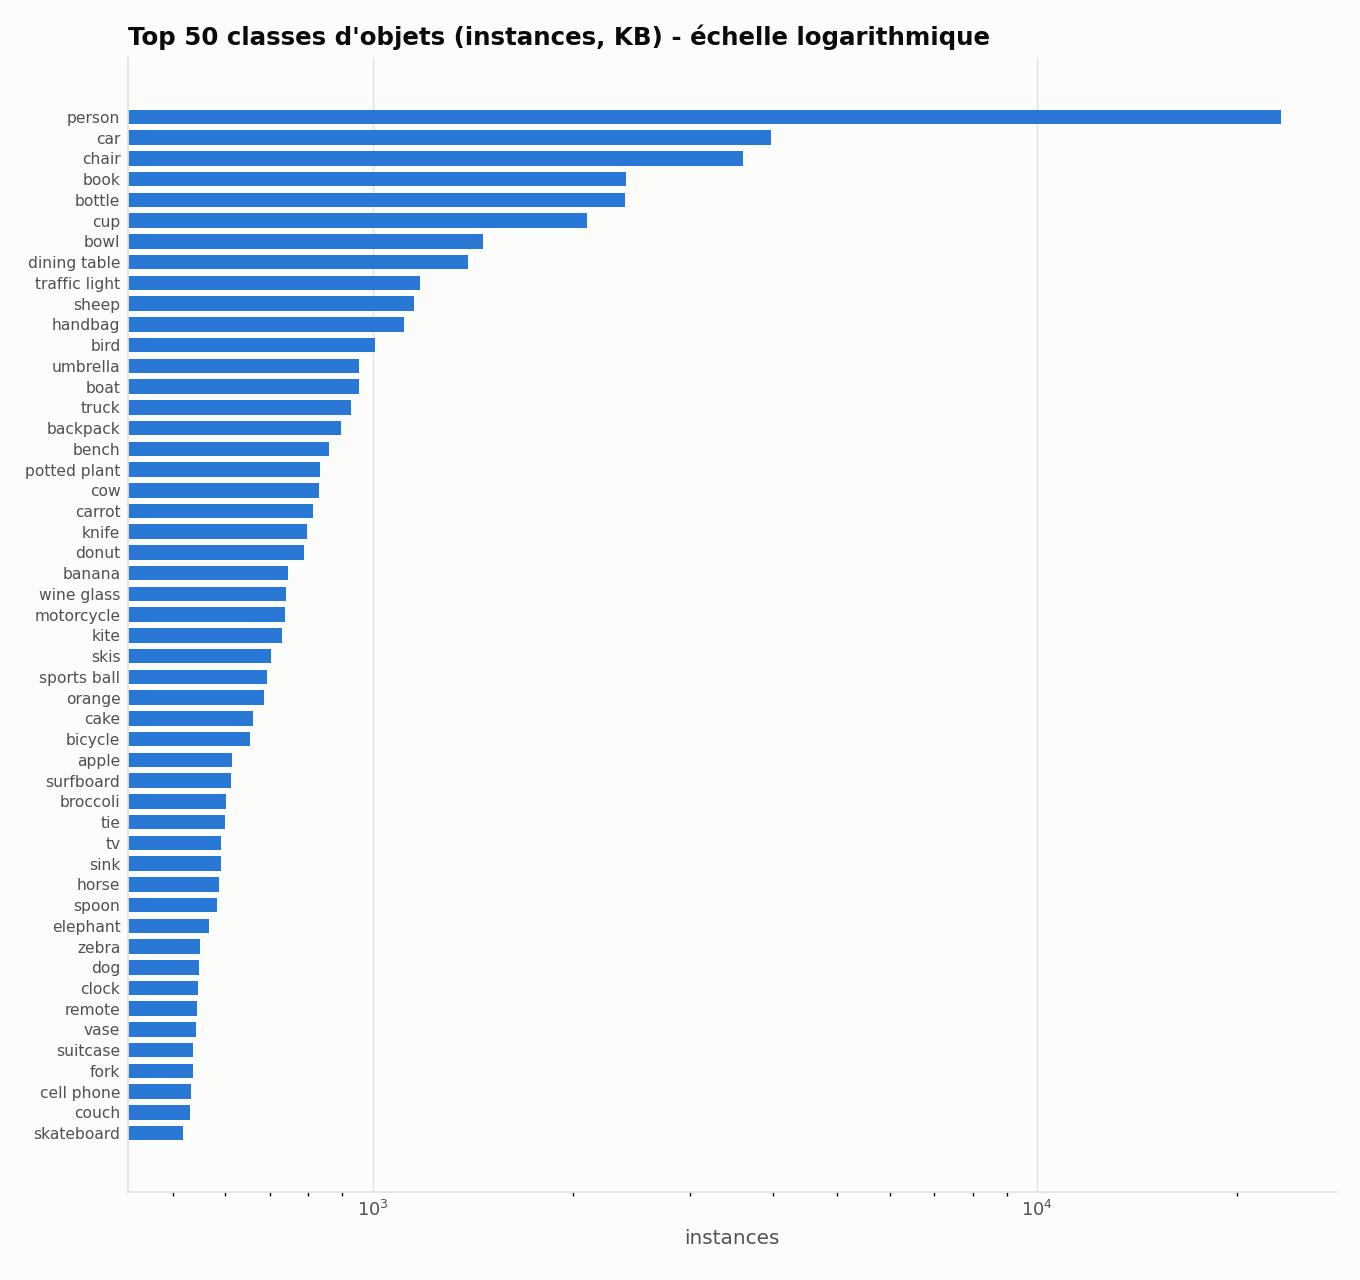
\includegraphics[width=0.85\textwidth]{../artifacts/eda/01_top50_classes.png}
\caption{The 50 most frequent classes in the KB. Values are stored in
\texttt{stats.json}, with person having 23,286 instances and appearing
in 5,599 images. Other prominent classes include car, chair, book,
bottle, cup, bowl, dining table, traffic light, and sheep.}
\label{fig:top50-classes}
\end{figure}

Person is the most frequent category in the KB, followed by classes
such as car, chair, book, and bottle. These statistics help describe
the dataset and identify common object categories.

\begin{figure}[htbp]
\centering
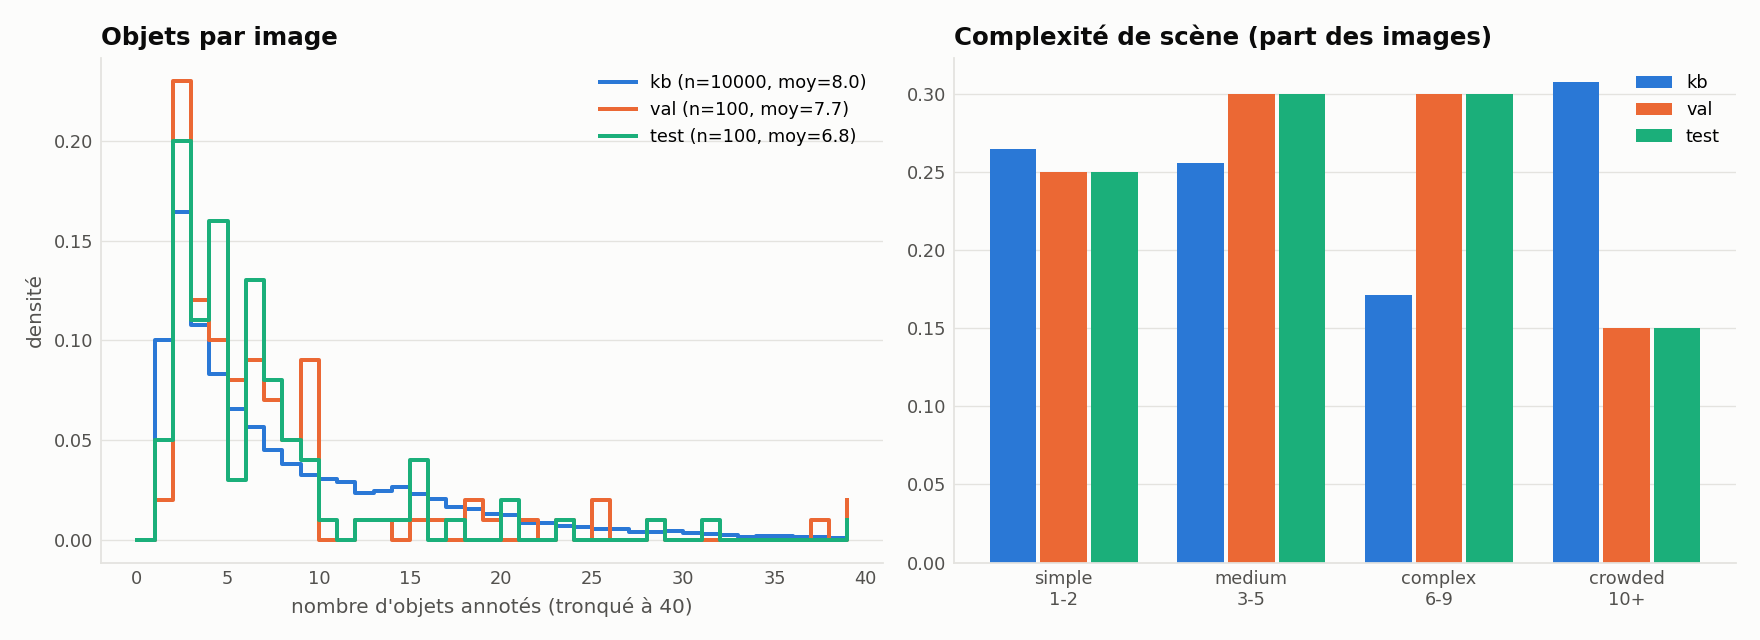
\includegraphics[width=0.85\textwidth]{../artifacts/eda/02_scene_complexity.png}
\caption{Scene-complexity distributions. The KB follows a natural
distribution (26.47\% simple, 25.61\% medium, 17.15\% complex, and 30.77\%
crowded), whereas validation and test follow the implemented
25/30/30/15\% quotas.}
\label{fig:scene-complexity}
\end{figure}

The difference between KB and test scene complexity is statistically
significant (\(\chi^2=18.3304\), \(p=0.000376\)). This difference is
expected because the KB keeps its natural distribution, while the
test set was deliberately balanced using the predefined
stratification targets.

\subsection{Spatial relations and
layout}\label{spatial-relations-and-layout}

Figure~\ref{fig:spatial-relations} presents geometric relation
frequencies. The repository derives relations by normalized bounding-box
geometry, not semantic scene understanding. Left-of and right-of are
complementary pair counts and occur at equal total frequencies, as do
above/below and inside/contains. In the KB, the proportions are 28.668\%
for left/right, 10.412\% for above/below, 10.351\% for overlapping,
4.758\% for inside/contains, and 1.973\% for on-top-of; note that each
inverse relation pair represents one stored relation in each directional
interpretation. The same pattern holds across evaluation splits.

\begin{figure}[htbp]
\centering
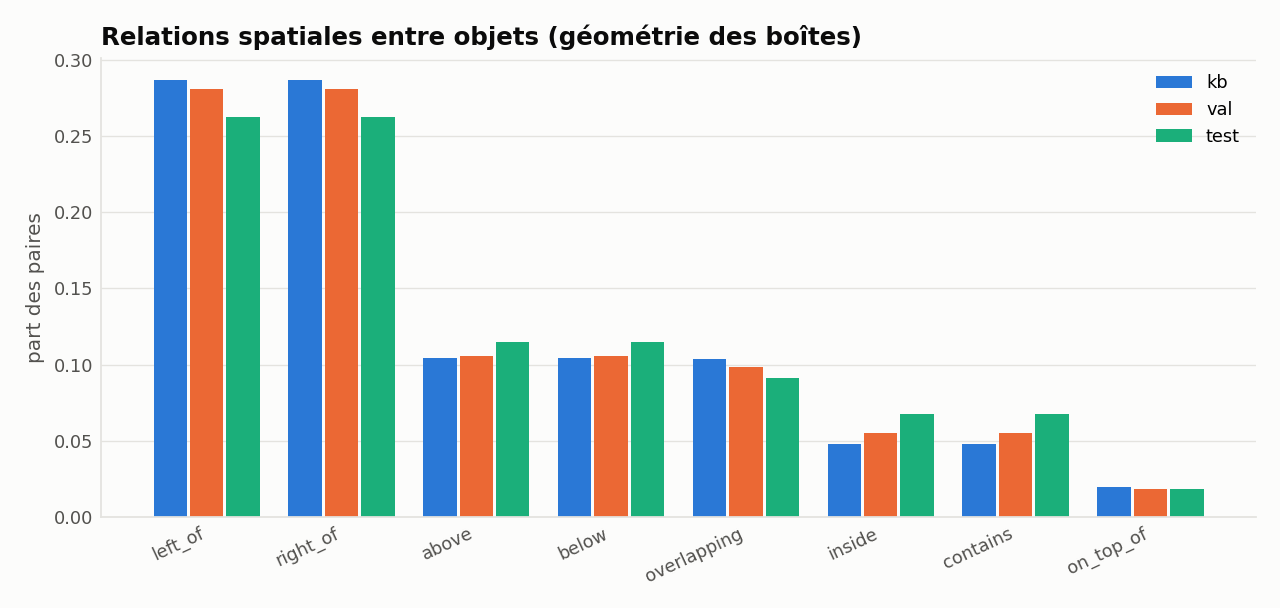
\includegraphics[width=0.85\textwidth]{../artifacts/eda/03_spatial_relations.png}
\caption{Spatial relations inferred from object bounding boxes. The
symmetry between directional relation pairs is geometric by construction.}
\label{fig:spatial-relations}
\end{figure}

\subsection{Captions and lexical
statistics}\label{captions-and-lexical-statistics}

Mean caption length is stable across splits: 10.483 KB tokens, 10.488
validation tokens, and 10.472 test tokens, with median 10 in every
split. The full KB vocabulary contains 9,697 unique tokens, 3,936 hapax
legomena, and 524,149 tokens. Token-level type-token ratios should not
be compared directly across split sizes, because the value for KB is
0.0185, versus 0.1844 and 0.1765 for validation and test. Validation has
967 vocabulary items and the test has 924. Out-of-vocabulary rates
relative to the KB are 1.09\% for validation and 0.74\% for test.

The repository compares KB and test caption lengths using a two-sample
Kolmogorov-Smirnov statistic of \(D=0.02484\),
\(p=0.9125\). This result supports the descriptive observation that
caption lengths are similar despite the intentionally different
stratification. Figure~\ref{fig:caption-length} combines
caption-length and Zipf-style evidence.

\begin{figure}[htbp]
\centering
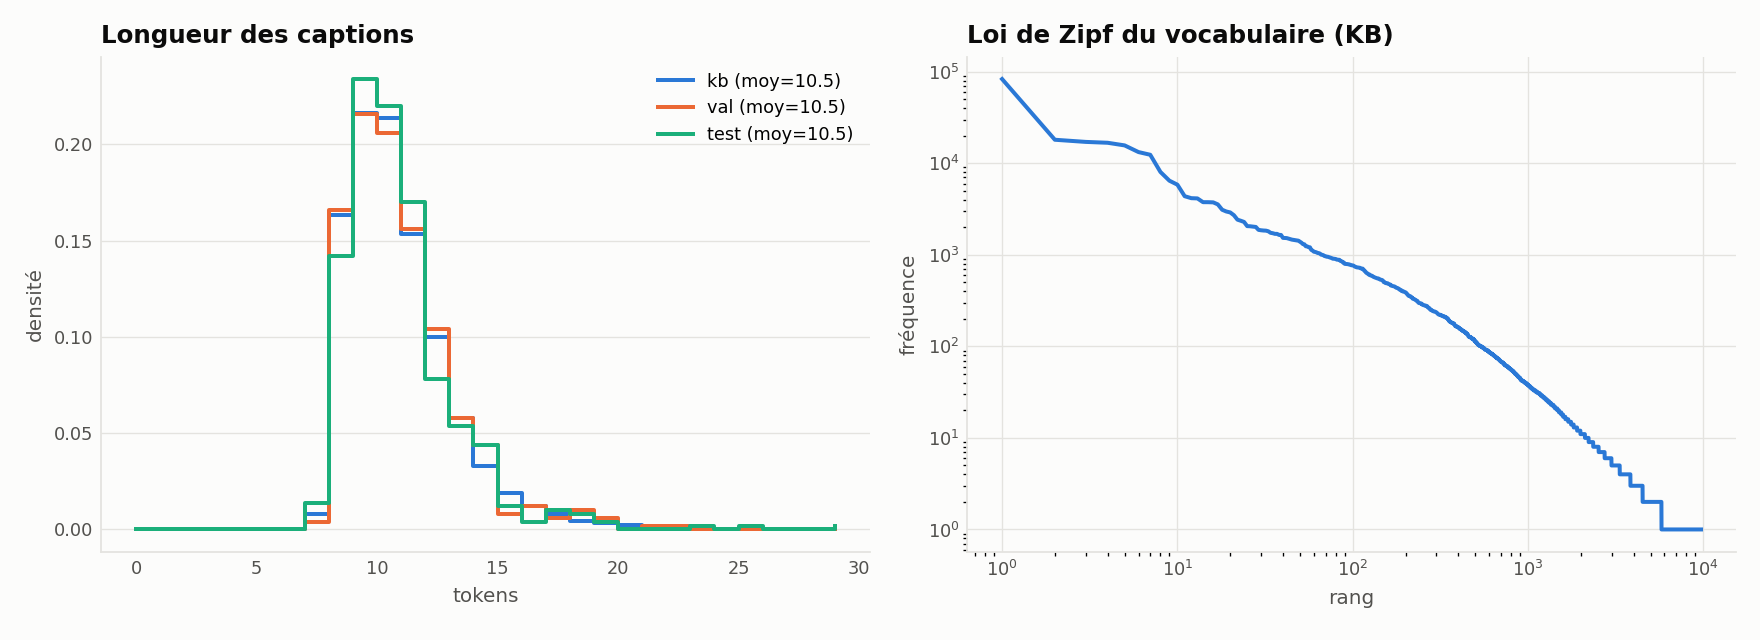
\includegraphics[width=0.85\textwidth]{../artifacts/eda/04_caption_length_zipf.png}
\caption{Caption-length distributions and associated corpus-frequency
visualization. The short caption bodies are concentrated around the same
median across all splits.}
\label{fig:caption-length}
\end{figure}

The NLTK part-of-speech distribution recorded for the KB has 74,604
nouns, 44,638 determiners, 33,596 prepositions, and 24,269 verbs, with
lower counts for adjectives, pronouns, conjunctions, numerals, adverbs,
particles, and unknown tags. Figure~\ref{fig:pos-distribution} displays the
distribution.

\begin{figure}[htbp]
\centering
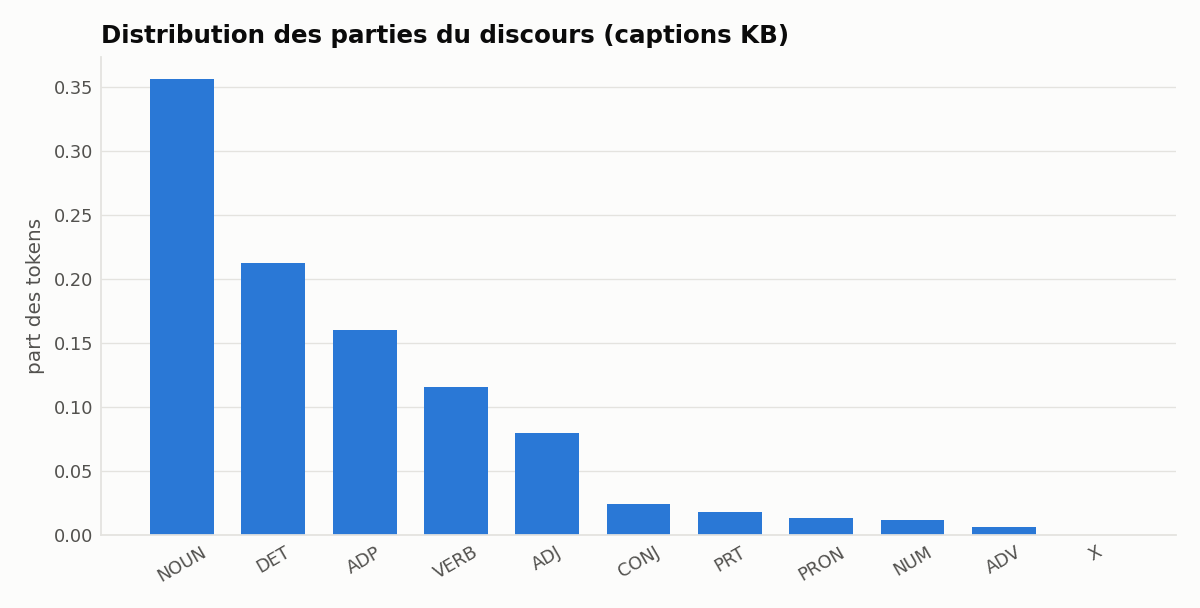
\includegraphics[width=0.85\textwidth]{../artifacts/eda/05_pos_distribution.png}
\caption{Part-of-speech distribution derived from the KB captions.}
\label{fig:pos-distribution}
\end{figure}

\subsection{Co-occurrence and image-text
association}\label{co-occurrence-and-image-text-association}

The repository analyses frequent class co-occurrence and the association
between object count and caption length. The recorded Spearman
correlation in the KB is \(\rho=0.13858\), with
\(p=4.5492\times10^{-44}\). Because the sample contains 50,000
captions, the correlation is statistically distinguishable from zero
despite its small descriptive magnitude. It should not be interpreted as
a direct causal relationship between scene object count and linguistic
richness.

Figure~\ref{fig:cooccurrence} visualizes the leading class
pairs. Figure~\ref{fig:objects-caption} displays the
relationship between annotation count and caption length.

\begin{figure}[htbp]
\centering
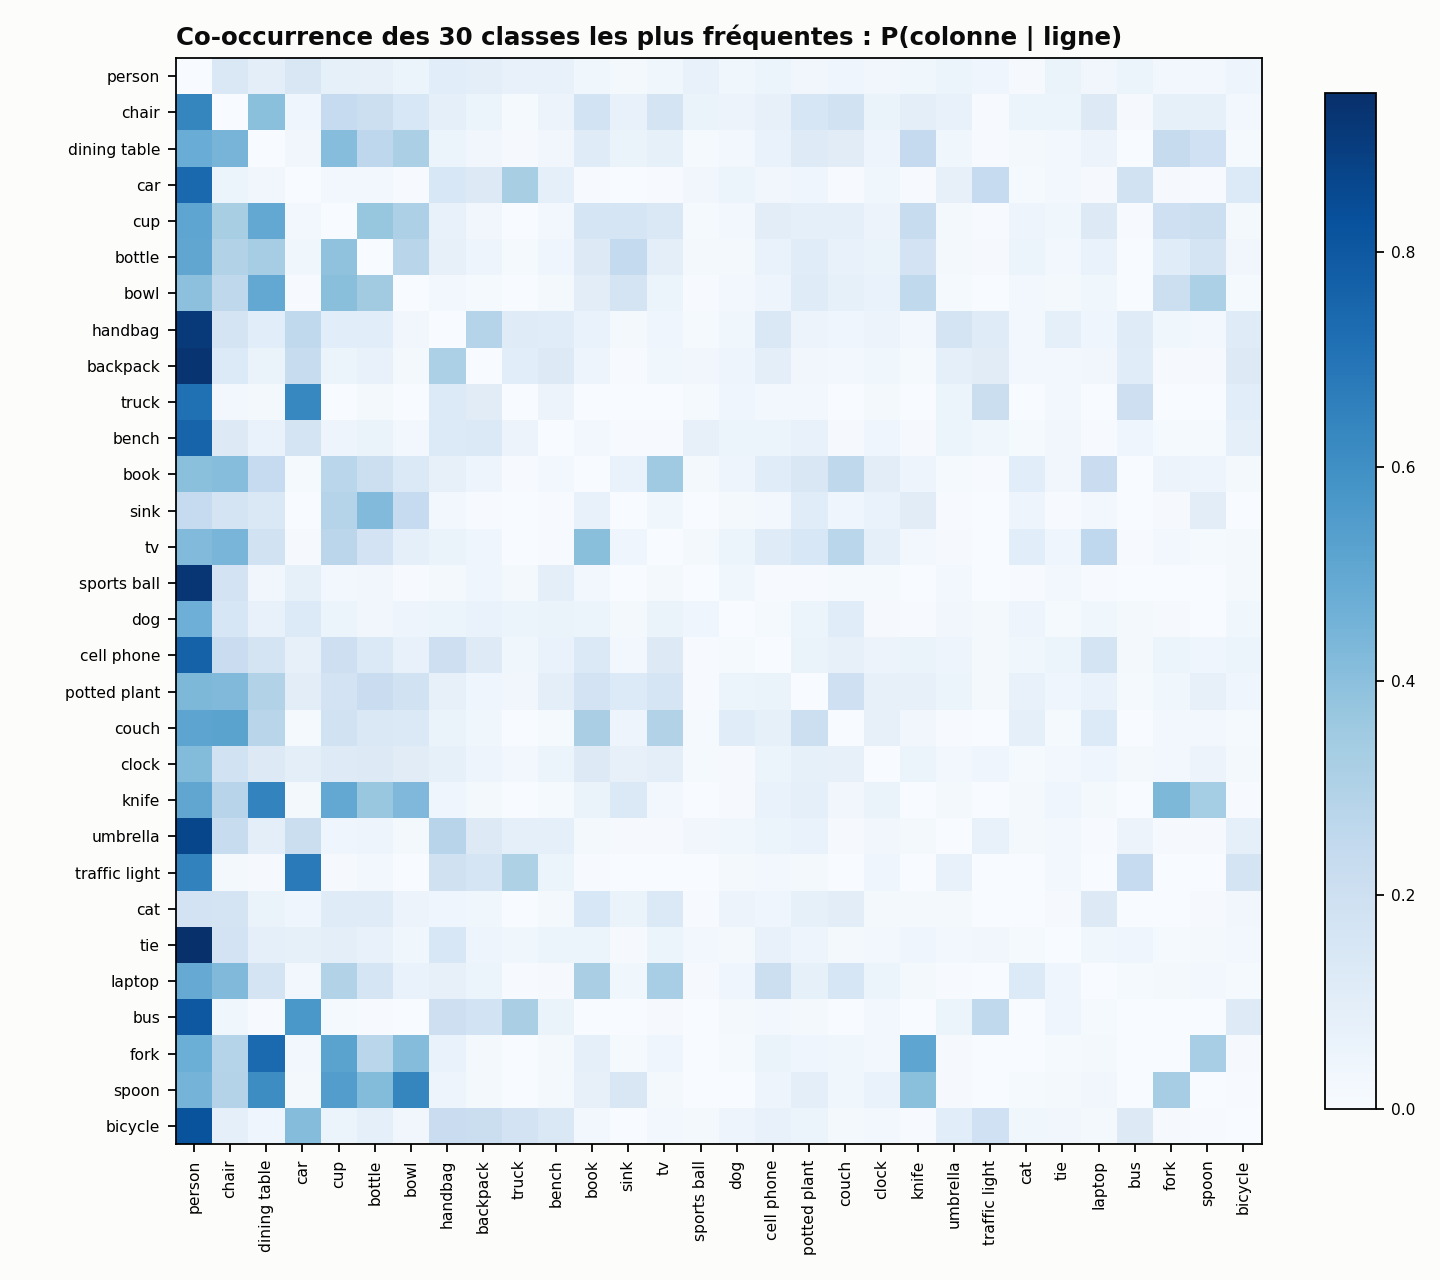
\includegraphics[width=0.85\textwidth]{../artifacts/eda/06_cooccurrence_top30.png}
\caption{Top 30 object-class co-occurrences in the KB.}
\label{fig:cooccurrence}
\end{figure}

\begin{figure}[htbp]
\centering
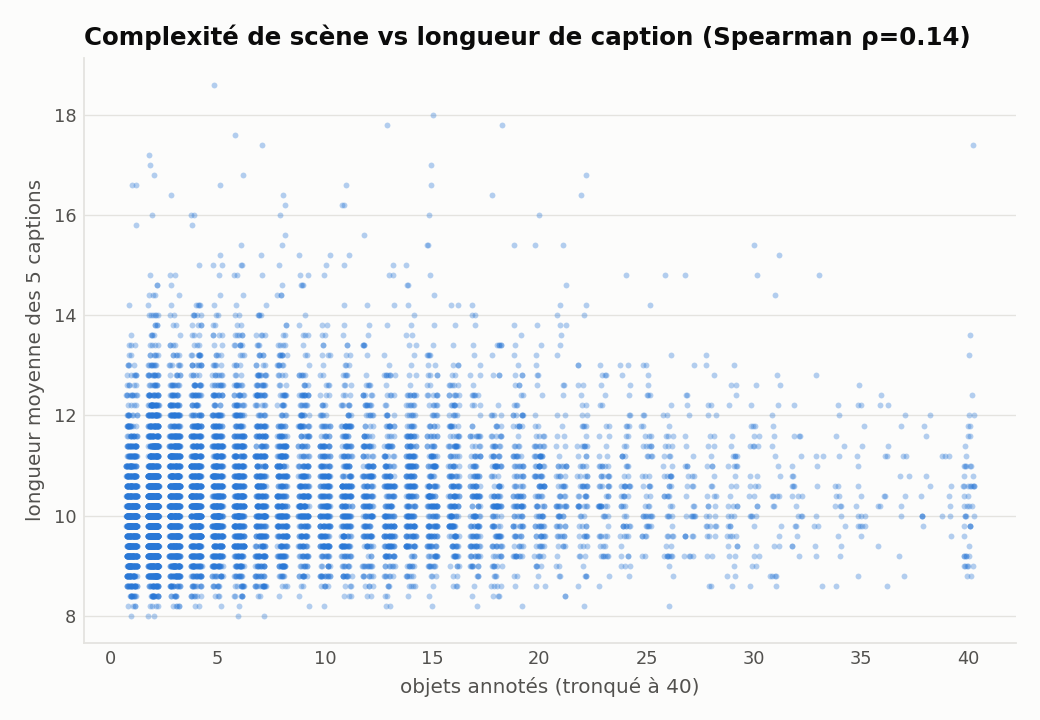
\includegraphics[width=0.85\textwidth]{../artifacts/eda/07_objects_vs_caption_length.png}
\caption{Relationship between object count and caption length.}
\label{fig:objects-caption}
\end{figure}

\subsection{Split
representativeness}\label{split-representativeness}

The Jensen-Shannon divergence of class distributions is 0.0311 for KB
versus validation and 0.0313 for KB versus test, in a convention where
zero denotes identical distributions. These small divergences indicate
broadly similar class populations. Nevertheless, they do not demonstrate
visual equivalence: validation and test are intentionally constrained
samples, and their allocation differs from the KB's natural
distribution.

All 80 classes occur in every split and the test has no missing class.
Thus class coverage is complete at the category level, although the
number of images representing each class in an evaluation split may be
modest. Figure~\ref{fig:diversity} summarizes context,
illumination, object size, and related diversity measures.

\begin{figure}[htbp]
\centering
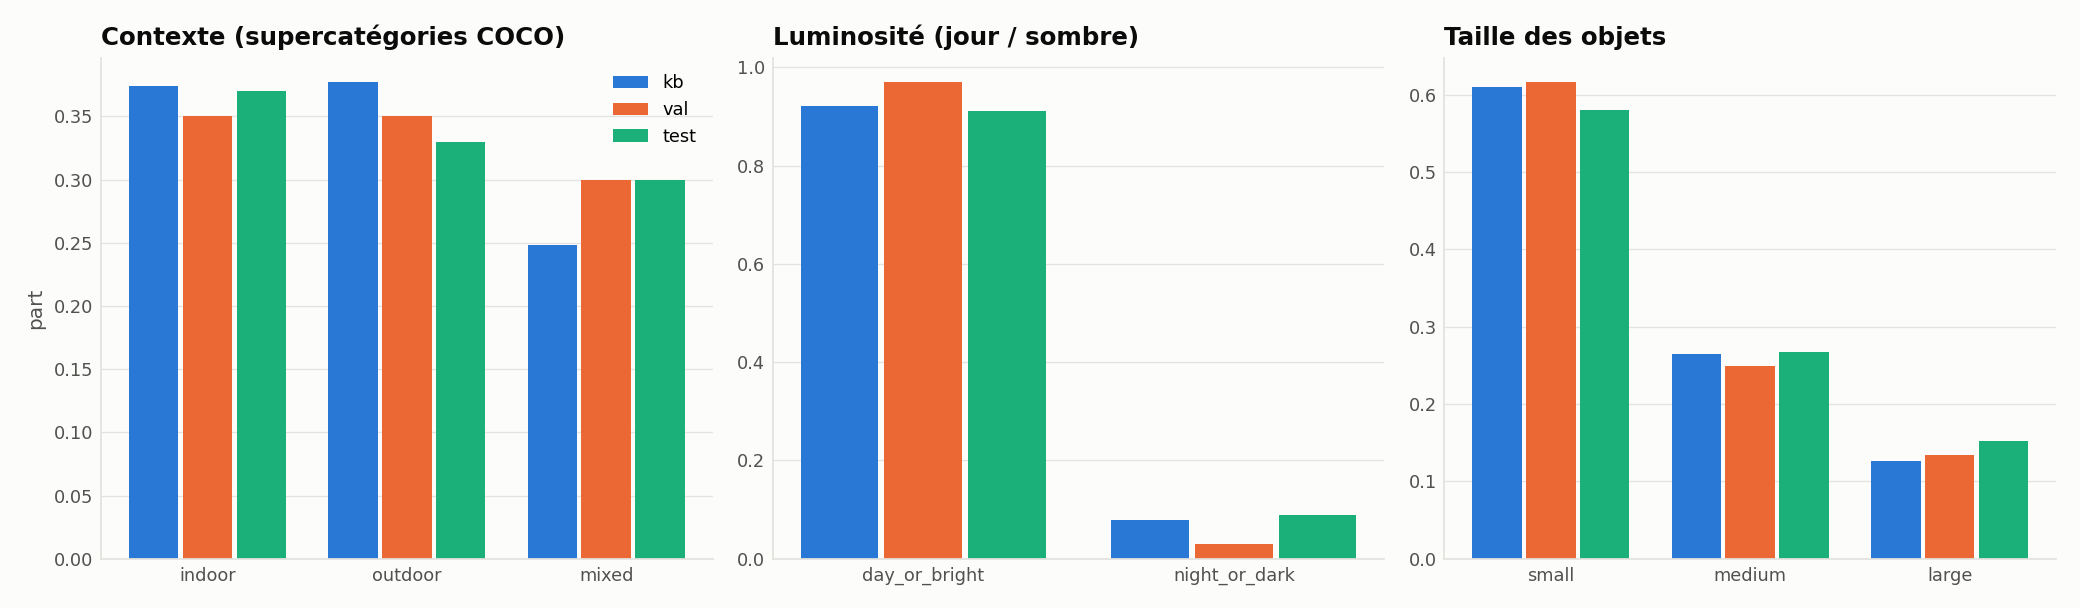
\includegraphics[width=0.85\textwidth]{../artifacts/eda/08_diversity_context_light_size.png}
\caption{Context and visual-diversity distributions across splits.}
\label{fig:diversity}
\end{figure}

In the KB, 92.16\% of images are day/bright; in validation and test the
corresponding shares are 97\% and 91\%. Gray is the leading dominant
image colour in all splits. KB object-size shares are approximately
60.95\% small, 26.42\% medium, and 12.64\% large.
Figure~\ref{fig:dominant-colours} presents the colour distribution and
Figure~\ref{fig:sample-grid} provides the qualitative image sample grid.

\begin{figure}[htbp]
\centering
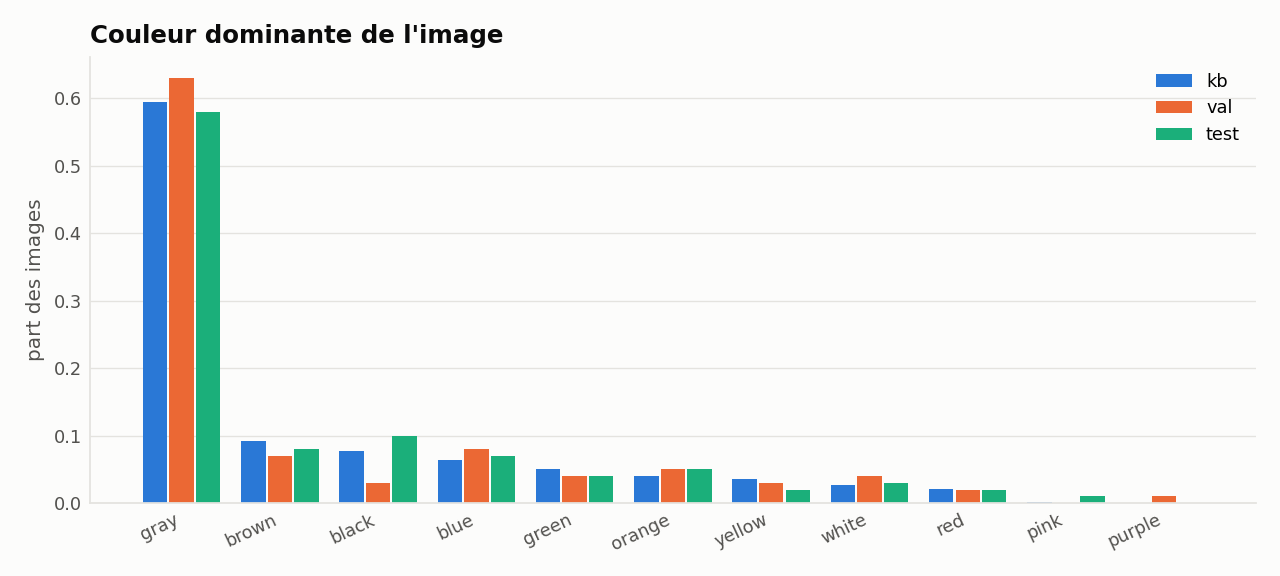
\includegraphics[width=0.85\textwidth]{../artifacts/eda/09_dominant_colors.png}
\caption{Dominant visual colours by split.}
\label{fig:dominant-colours}
\end{figure}

\begin{figure}[p]
\centering
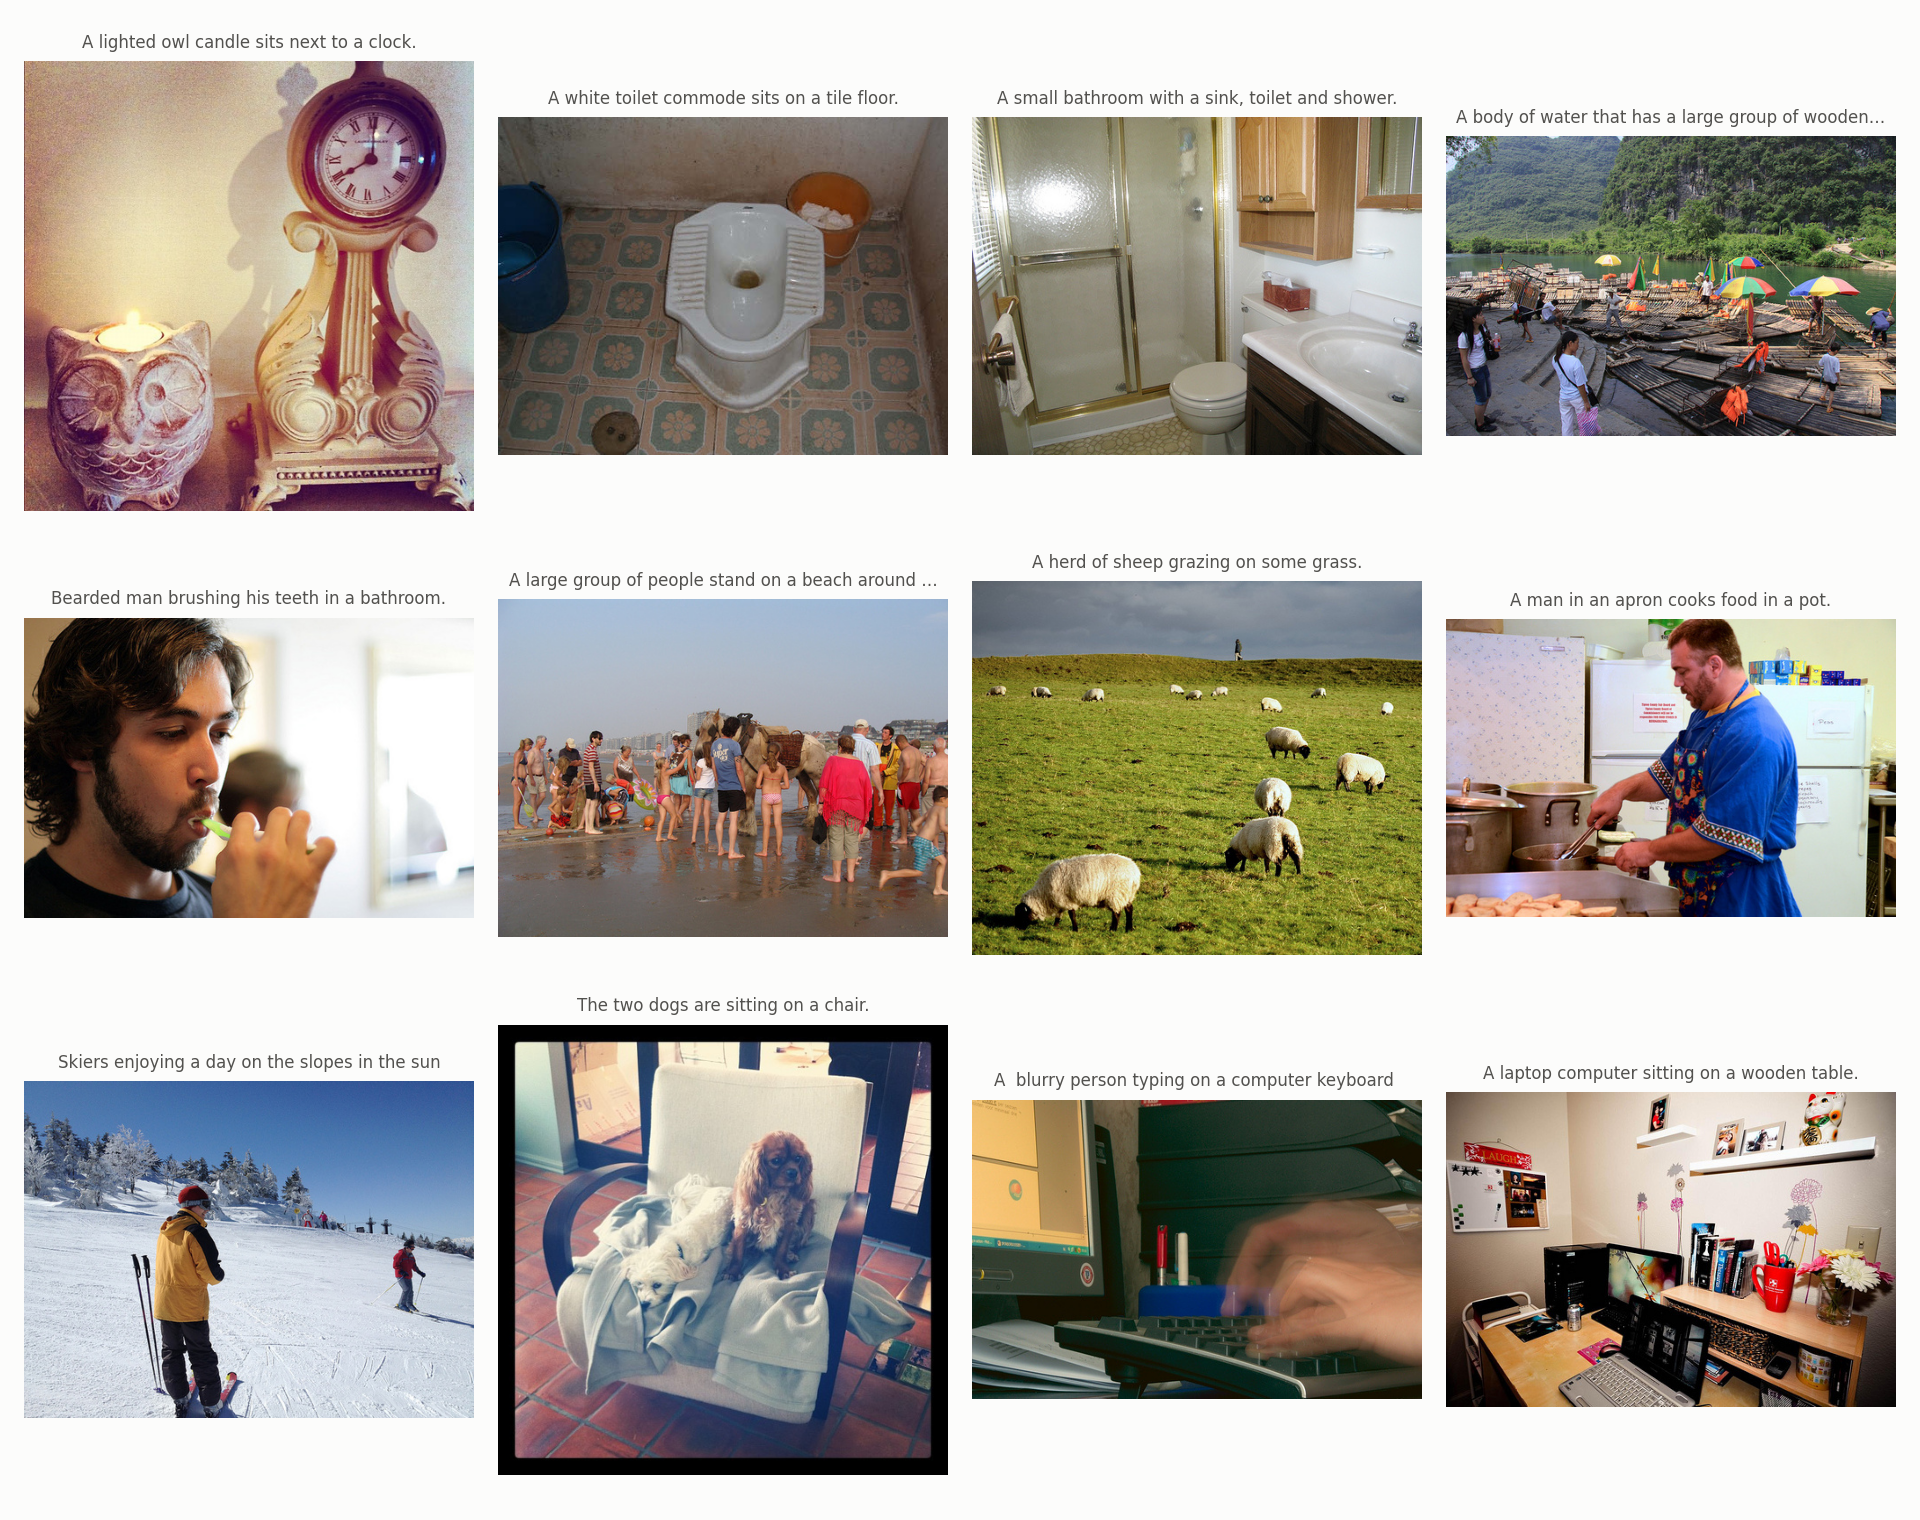
\includegraphics[width=\textwidth,height=0.72\textheight,keepaspectratio]{../artifacts/eda/10_sample_grid.png}
\caption{Qualitative sample from the frozen release.}
\label{fig:sample-grid}
\end{figure}

Finally, the fixed caption attribute lexicon identifies colour, size,
material, state, and shape expressions in KB captions. Its largest
recorded category counts are 10,586 colour, 5,604 size, 2,532 state,
1,766 material, and 239 shape attributes. White is the most frequent
colour attribute with 2,943 occurrences, followed by large and small.
Shape counts include flat 73, round 57, square 53, circular 14,
rectangular 12, and oval 9 occurrences in the figure's source data.
Figure~\ref{fig:caption-attributes} illustrates these distributions.

\begin{figure}[htbp]
\centering
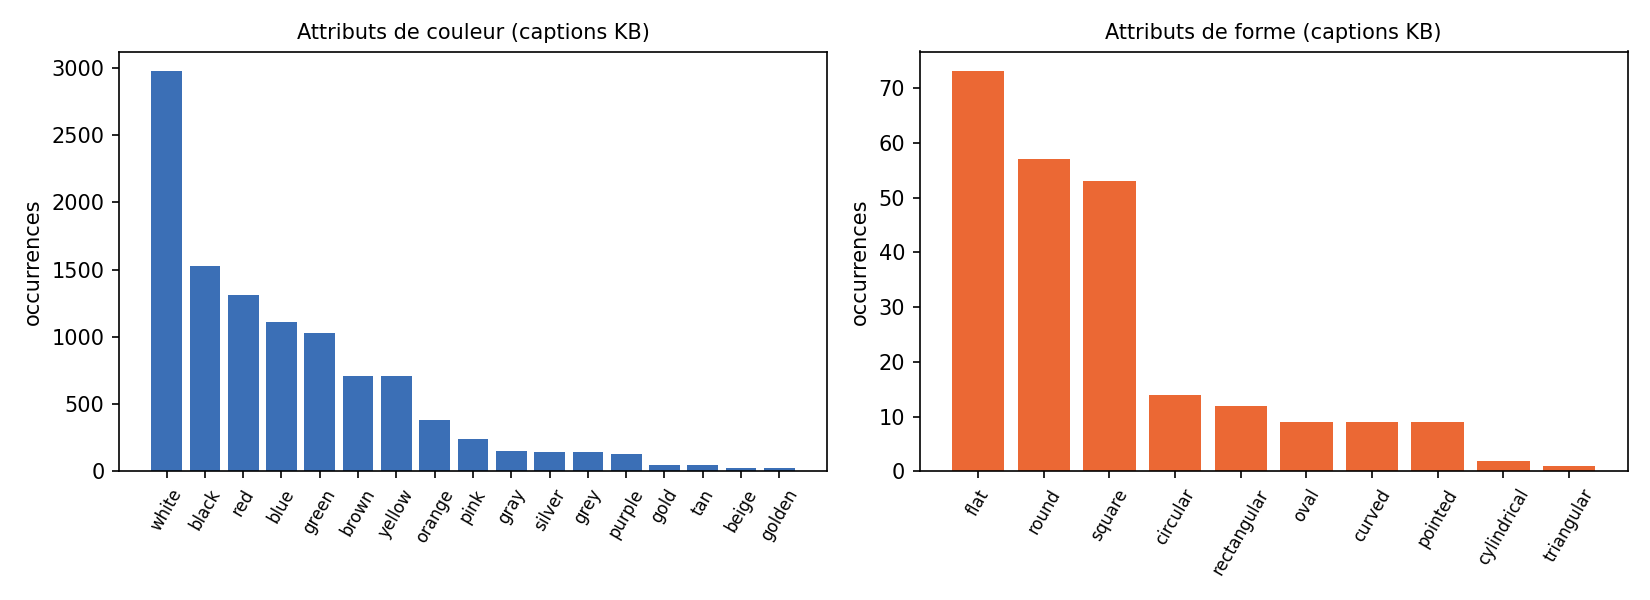
\includegraphics[width=0.85\textwidth]{../artifacts/eda/11_attributs_couleur_forme.png}
\caption{Distribution of lexical colour and shape attributes in KB
captions.}
\label{fig:caption-attributes}
\end{figure}

\newpage
\section{Image and Caption
Preprocessing}\label{image-and-caption-preprocessing}

\subsection{Image normalization}\label{image-normalization}

Each image is checked for validity and converted to RGB format.
Images larger than 512 pixels on their longest side are resized while
preserving their aspect ratio. Smaller images are not enlarged.

Images are saved as JPEG files with quality 95. The pipeline also
records image dimensions, colour information, brightness, sharpness,
and file hashes for quality control.

\subsection{Model-specific
preprocessing}\label{model-specific-preprocessing}

Each model uses its own preprocessing tools. CLIP and SigLIP use
their Hugging Face processors to prepare images and text, while
DINOv2 uses its image processor and CLS token to extract image
features.

CLIP uses a maximum text length of 77 tokens, while SigLIP uses
64 tokens.

\subsection{Caption cleaning}\label{caption-cleaning}

For each KB image, the first five captions are selected and stored.
The raw captions are preserved, while cleaned versions are converted
to lowercase, stripped of unnecessary characters, and normalized
for whitespace.

Evaluation captions remain separate from the KB to prevent evaluation
references from being included in retrieval data

\section{Metadata Extraction}\label{metadata-extraction}

Each split is joined to COCO instance annotations and caption records.
Crowd annotations are ignored. For every non-crowd object, the pipeline
records COCO category identity and supercategory, normalized
bounding-box coordinates, image-area fraction, and size:

\[
\text{small}:a<0.02,\quad
\text{medium}:0.02\leq a<0.15,\quad
\text{large}:a\geq0.15,
\]

where \(a\) is the object bounding-box area fraction after clipping to
image bounds. For the largest objects, the pipeline estimates a named
pixel colour for objects with area fraction at least 0.01, processing up
to eight objects.

Top-level metadata also includes category counts, object counts,
supercategories, complexity, context, day/night status, brightness,
colorfulness, dominant colours, relations, and KB caption attributes.
Complexity follows the thresholds in Section 3. Context is assigned
through indoor/outdoor COCO supercategories. Day/night is based on the
configured brightness threshold of 0.28.

Eight geometric relations---`inside`, `contains`, `on\_top\_of`,
`overlapping`, `left\_of`, `right\_of`, `above`, and `below`---are
calculated from bounding-box geometry among the largest objects. They
are not inferred by a semantic scene graph. Caption attributes come from
fixed lexicons of 17 colours, 8 materials, 10 size words, 13 states, and
shape expressions.

For implementation realism, the repository's optional DETR path can
supply predicted object detections. However, frozen validation/test
objects in `metadata.jsonl` are COCO ground truth and therefore
constitute an oracle for evaluating query metadata. This limitation is
recorded explicitly and must be considered when interpreting downstream
metadata-based results.

\section{Data Quality Assessment and Anti-Leakage
Measures}\label{data-quality-assessment-and-anti-leakage-measures}

\subsection{Image audit and repair}\label{image-audit-and-repair}

The image audit confirms that all 10,200 images are readable and
valid. It also checks image formats, exact duplicates, and
near-duplicates.

Two duplicate images were identified in the KB: one exact duplicate
and one near-duplicate. Both were removed and replaced with other
images. The final audit found no remaining duplicates or qualifying
near-duplicates under the configured thresholds.

\subsection{Cross-split identity
controls}\label{cross-split-identity-controls}

The three splits contain separate image IDs, and their integrity is
verified using SHA-256 hashes. The retrieval API also prevents a
query image from being returned as its own result.

Additional SigLIP similarity and difference-hash checks found no
qualifying near-duplicates between the evaluation sets and the KB.

Table 4 summarizes the QC programme rather than
reproducing all 40 individual rows.

\begin{center}
\textbf{Table 4. Consolidated quality-control outcome.}
\end{center}
\label{tab:qc}

\begin{table}[htbp]
\centering
\begin{tabular}{lp{9.2cm}}
\toprule
QC area & Result \\
\midrule
Split identity and counts & 40 checks executed; 40 passed \\
Invalid images & 0 \\
Exact duplicates & 0 \\
Validation/test near-duplicates & 0/100 in each split using SigLIP cosine and dHash \\
KB caption coverage & Exactly 5 caption rows/image \\
Evaluation reference coverage & Exactly 5 rows/image \\
Embeddings and indexes & Sizes aligned to split and embedding dimensions \\
Retrieval smoke tests & Passed for validation and test \\
\bottomrule
\end{tabular}
\end{table}

Table 4 should be read together with the detailed repository audit. The
frozen report contains 40 checks, no failures, and no warnings.

\subsection{Caption-string overlap}\label{caption-string-overlap}

The QC normalized evaluation captions and KB captions with the same
cleaning function. It found normalized string matches on 5 of 500
validation reference rows (1.0\%) and 7 of 500 test reference rows
(1.4\%). Those matches involved 9 and 37 evaluation-image-to-KB-image
mappings, respectively, because generic descriptions occur on multiple
KB images.

This result is not interpreted as image leakage. Every listed pair has
different evaluation and KB image IDs, and clean-string equality alone
does not establish that either the underlying image or a source caption
record leaked across splits. The audit explicitly reports these
occurrences so that repetitive generic captions do not conceal their
presence.

\section{Image and Text Embeddings}\label{image-and-text-embeddings}

The pipeline generates image and text embeddings using four models:
CLIP \cite{radford_learning_2021}, SigLIP \cite{zhai_sigmoid_2023},
DINOv2 \cite{oquab_dinov2_2023}, and Sentence-BERT
\cite{reimers_sentence-bert_2019}. These embeddings represent
images and captions as numerical vectors that can be compared using
similarity measures.

All embeddings are stored as normalized float32 vectors. Table 5
summarizes the dimensions and number of vectors generated by each
model.

\begin{center}
\textbf{Table 5. Embedding products and frozen shapes.}
\end{center}

\begin{table}[htbp]
\centering
\begin{tabular}{lrrr}
\toprule
Product & Image KB & Val/test images & Text KB \\
\midrule
CLIP ViT-B/32 & \(10{,}000\times512\) & \(100\times512\) & \(50{,}000\times512\) \\
SigLIP base patch16/224 & \(10{,}000\times768\) & \(100\times768\) & \(50{,}000\times768\) \\
DINOv2-small & \(10{,}000\times384\) & \(100\times384\) & --- \\
SBERT all-MiniLM-L6-v2 & --- & --- & \(50{,}000\times384\) \\
\bottomrule
\end{tabular}
\end{table}

Table 5 demonstrates aligned vector dimensions within each image/text
space and fixed row alignment with image and caption IDs. CLIP and
SigLIP support both image-to-image and image-to-text retrieval. DINOv2
supports only image vectors in the frozen release, while SBERT supplies
a separate caption embedding not linked to a FAISS index in this
release.

For vectors \(\mathbf x,\mathbf y\), normalization permits cosine
similarity to be computed as

\begin{equation*}
\cos(\mathbf{x},\mathbf{y})
=\frac{\mathbf{x}^{\top}\mathbf{y}}
       {\|\mathbf{x}\|_{2}\|\mathbf{y}\|_{2}}
\approx \mathbf{x}^{\top}\mathbf{y},
\qquad \|\mathbf{x}\|_{2}=\|\mathbf{y}\|_{2}=1.
\end{equation*}

An inner-product index operating on L2-normalized vectors implements cosine-similarity retrieval.

\section{Knowledge Base and FAISS Index
Construction}\label{knowledge-base-and-faiss-index-construction}

\subsection{Exact image and text
indexes}\label{exact-image-and-text-indexes}

FAISS \cite{johnson_billion-scale_2021} is used to build similarity-search indexes for the KB.
The image indexes contain 10,000 vectors each, while the CLIP and
SigLIP text indexes contain 50,000 caption vectors each.

The indexes use IndexFlatIP, which performs exact inner-product
search. Since the vectors are normalized, this is equivalent to
cosine similarity. 

Table 6 summarizes the index configurations
and their build times.

\begin{center}
\textbf{Table 6. Image FAISS index configurations.}
\end{center}
\label{tab:indexes}

\begin{table}[htbp]
\centering
\resizebox{\textwidth}{!}{\begin{tabular}{lrrrrrp{4cm}}
\toprule
Encoder & Dimension & Flat size & Flat build & HNSW size & HNSW build & Parameters \\
\midrule
CLIP & 512 & 20.480 MB & 0.0081 s & 23.198 MB & 4.0060 s & \(M=32\), efConstruction 200, efSearch 64 \\
DINOv2 & 384 & 15.360 MB & 0.0497 s & 18.078 MB & 6.8016 s & \(M=32\), efConstruction 200, efSearch 64 \\
SigLIP & 768 & 30.720 MB & 0.0225 s & 33.438 MB & 1.4390 s & \(M=32\), efConstruction 200, efSearch 64 \\
\bottomrule
\end{tabular}}
\end{table}

Table 6 makes clear that storage grows primarily with vector dimension
rather than the same number of vectors multiplied by byte width. The
flat image-index build measurements are reported by
`index\_report.json`; however, they are not comparable to the separate
NumPy latency benchmark used in encoder comparison scripts.

The CLIP and SigLIP caption indexes are 512- and 768-dimensional
`IndexFlatIP` structures containing 50,000 vectors. Filesystem sizes are
102,400,045 bytes and 153,600,045 bytes, respectively. The index report
does not record separate text-index build times or MB values, so no
value is inferred for those fields.

\subsection{Approximate HNSW search}\label{approximate-hnsw-search}

HNSW indexes provide faster approximate similarity search.
They use M=32, efConstruction=200, and efSearch=64.

Recall@10 is 1.000 for CLIP, 0.997 for DINOv2, and 0.999 for
SigLIP, showing that approximate search closely matches exact
search. For SigLIP, median search latency decreases from 0.737 ms
with flat search to 0.082 ms with HNSW.

\subsection{Retrieval API}\label{retrieval-api}

The public `Release` class loads the configured encoder, performs image
and caption retrieval, and maps returned KB IDs to raw captions. Flat
and HNSW image indexes are separately addressable. A query with supplied
`query\_ids` is checked against every returned ID and raises an error if
its own image is returned. For the image-to-text mode, query vectors are
searched against the 50,000 caption vectors and aligned parent-image IDs
are returned.


\newpage

\section{Encoder Comparison and Validation-Based
Selection}\label{encoder-comparison-and-validation-based-selection}

\subsection{Retrieval
configurations}\label{retrieval-configurations}

Five retrieval configurations are compared using CLIP, DINOv2,
and SigLIP.

In image-to-image retrieval, the query image is compared with KB
images, and the caption of the most similar image is returned.
In image-to-text retrieval, the query image is compared directly
with KB caption embeddings to retrieve the most similar caption.

The configurations are evaluated using retrieval metrics and CIDEr \cite{vedantam_cider_2015}.
A random-caption baseline is also included for comparison.

\subsection{Validation selection
metric}\label{validation-selection-metric}

CIDEr \cite{vedantam_cider_2015} is used as the main metric for selecting the best
configuration. Each configuration is evaluated on the 100
validation images, and the one with the highest mean CIDEr is
selected. Jaccard class@1 is used as a tie-breaker.

SigLIP image-to-text achieves the highest validation CIDEr of
0.7223 and is therefore selected. The test set is kept separate
and is used only for final reporting.


\[
\text{selected} = \arg\max_c
\frac{1}{100}\sum_{i=1}^{100}\mathrm{CIDEr}(c,i).
\]

The selection was made before looking at the final test results. Test
data were retained in Table 9 and were not included in
configuration selection.

\section{Experimental Results and Statistical
Analysis}\label{experimental-results-and-statistical-analysis}

\subsection{Validation results}\label{validation-results}

Table 7 gives the validation metrics
recorded in the comparison artifact and repository CSV.

\begin{center}
\textbf{Table 7. Validation configuration comparison.}
\end{center}

\begin{table}[htbp]
\centering
\resizebox{\textwidth}{!}{\begin{tabular}{lrrrrrr}
\toprule
Configuration & Recall@1 & Recall@5/@10 & Precision@1/@5/@10 & MRR & Jaccard@1 & CIDEr \\
\midrule
SigLIP image-to-text & 0.96 & 1.00 / 1.00 & 0.96 / 0.972 / 0.962 & 0.9775 & 0.4994 & \textbf{0.7223} \\
SigLIP image-to-image & 1.00 & 1.00 / 1.00 & 1.00 / 0.976 / 0.969 & 1.0000 & 0.5455 & 0.6735 \\
CLIP image-to-text & 0.97 & 1.00 / 1.00 & 0.97 / 0.972 / 0.970 & 0.9850 & 0.5349 & 0.5584 \\
DINOv2 image-to-image & 0.98 & 1.00 / 1.00 & 0.98 / 0.960 / 0.961 & 0.9900 & 0.5209 & 0.5541 \\
CLIP image-to-image & 0.98 & 1.00 / 1.00 & 0.98 / 0.972 / 0.951 & 0.9883 & 0.5382 & 0.5286 \\
\bottomrule
\end{tabular}}
\end{table}

Table 7 shows that SigLIP image-to-text achieves the highest
validation CIDEr score of 0.7223. However, SigLIP image-to-image
achieves better recall@1 and MRR. This shows that retrieval
accuracy and caption quality do not always produce the same ranking.

The reported confidence intervals, mean differences, and Wilcoxon
comparisons against SigLIP image-to-text are reproduced in Table 8.

\begin{center}
\textbf{Table 8. Validation statistical comparison with SigLIP
image-to-text.}
\end{center}

\begin{table}[htbp]
\centering
\begin{tabular}{lrrrr}
\toprule
Configuration & Mean CIDEr & 95\% CI & Difference vs.\ best & Wilcoxon \(p\) \\
\midrule
SigLIP image-to-text & 0.7223 & [0.6168, 0.8387] & --- & --- \\
SigLIP image-to-image & 0.6735 & [0.5753, 0.7825] & 0.0487 & 0.3023 \\
CLIP image-to-text & 0.5584 & [0.4626, 0.6585] & 0.1638 & 0.00405 \\
DINOv2 image-to-image & 0.5541 & [0.4695, 0.6516] & 0.1682 & 0.01117 \\
CLIP image-to-image & 0.5286 & [0.4384, 0.6233] & 0.1937 & 0.00915 \\
\bottomrule
\end{tabular}
\end{table}

Table 8 presents the statistical comparison between the selected
configuration and the alternatives. SigLIP image-to-image is not
significantly different from SigLIP image-to-text
(\(p=0.3023\)). The other three configurations are significantly
lower under the Bonferroni-adjusted significance threshold (0.05/4 = 0.0125) \cite{cohen_statistical_2013}.

Therefore, SigLIP image-to-text is selected based on its highest
validation CIDEr, although its advantage over SigLIP image-to-image
is not statistically significant.

\subsection{Final test reporting}\label{final-test-reporting}

Table 9 presents report-only test values.
These results are not used to select a configuration.

\begin{center}
\textbf{Table 9. Report-only test results.}
\end{center}
\label{tab:test-results}

\begin{table}[htbp]
\centering
\resizebox{\textwidth}{!}{\begin{tabular}{lrrrrrr}
\toprule
Configuration & Recall@1 & Recall@5/@10 & Precision@1/@5/@10 & MRR & CIDEr & Random CIDEr \\
\midrule
CLIP image-to-image & 0.93 & 1.00 / 1.00 & 0.93 / 0.926 / 0.905 & 0.9567 & 0.6118 & 0.0420 \\
CLIP image-to-text & 0.96 & 1.00 / 1.00 & 0.96 / 0.960 / 0.957 & 0.9770 & 0.6501 & 0.0420 \\
DINOv2 image-to-image & 0.98 & 1.00 / 1.00 & 0.98 / 0.948 / 0.951 & 0.9870 & 0.5503 & 0.0420 \\
SigLIP image-to-image & 0.95 & 0.99 / 1.00 & 0.95 / 0.956 / 0.953 & 0.9717 & 0.6216 & 0.0420 \\
SigLIP image-to-text & 0.98 & 1.00 / 1.00 & 0.98 / 0.964 / 0.972 & 0.9883 & \textbf{0.7064} & 0.0420 \\
\bottomrule
\end{tabular}}
\end{table}

Table 9 presents the results on the legacy 100-image test. SigLIP
image-to-text achieves the highest CIDEr score of 0.7064, followed by CLIP
image-to-text at 0.6501. The random-caption baseline scores 0.0420.
The official 1,000-image test is reported in Section~\ref{official-test-results}.

These results are used only for final reporting and do not influence
the configuration selected using validation data.

Figure~\ref{fig:encoder-comparison} visualizes validation
CIDEr by configuration. The repository has one encoder-comparison chart,
named `encoder\_comparison\_val.png`.

\begin{figure}[htbp]
\centering
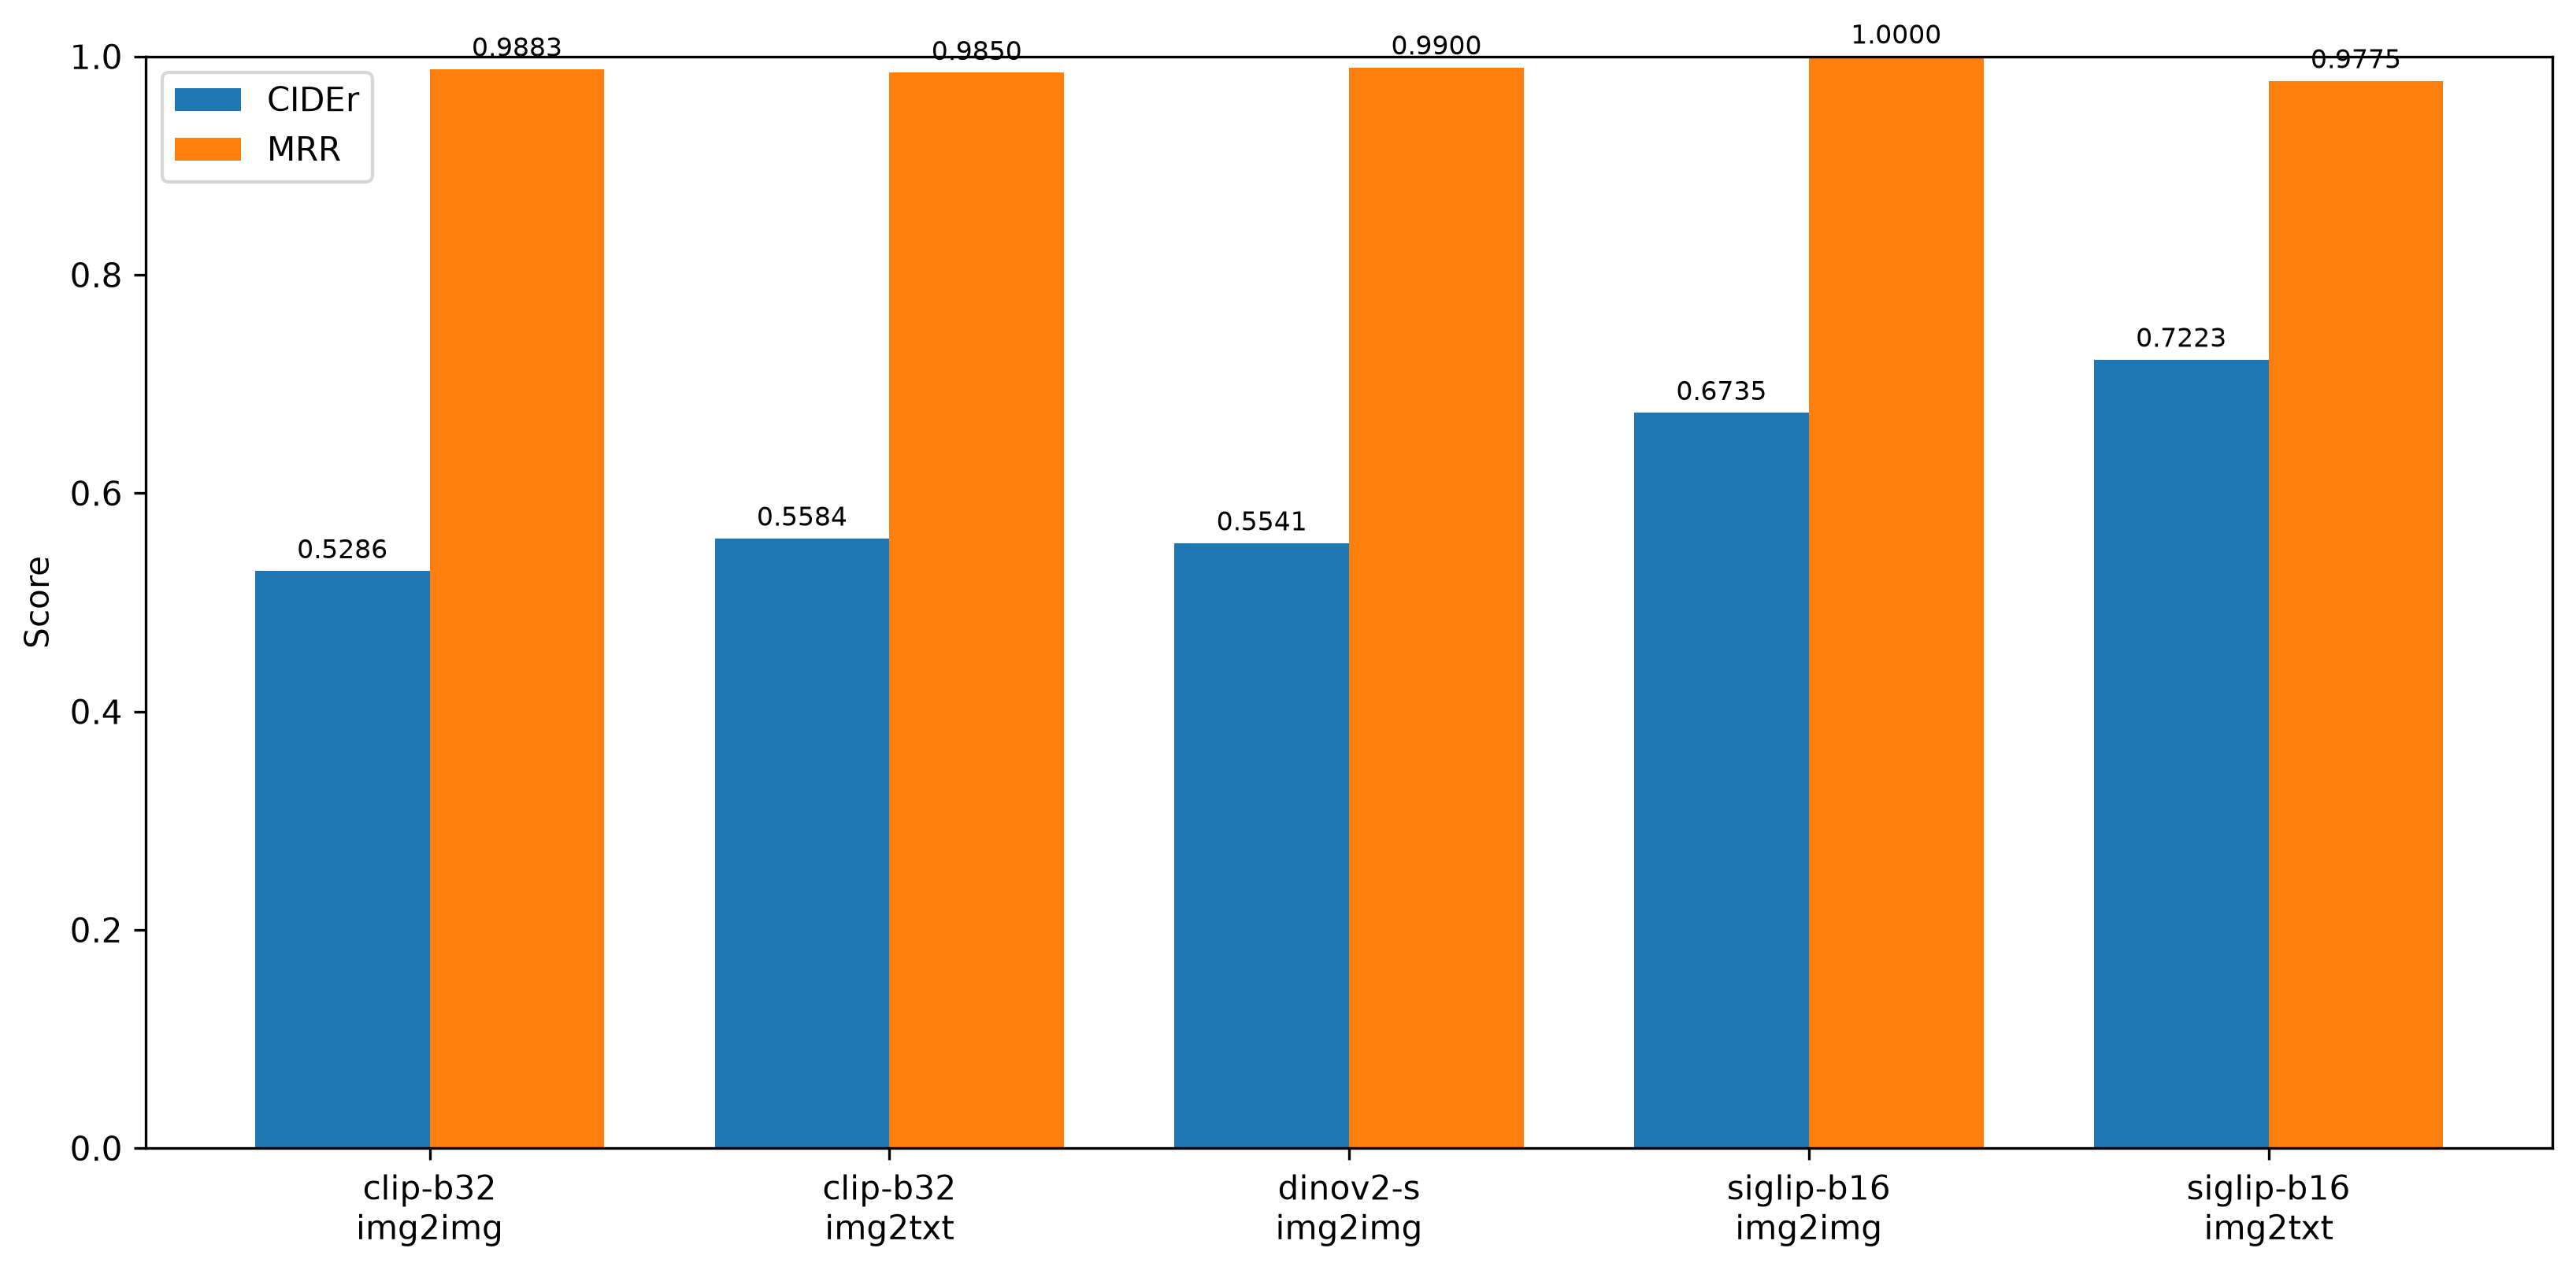
\includegraphics[width=0.85\textwidth]{encoder_comparison_val.png}
\caption{Validation CIDEr comparison for the five implemented retrieval
configurations.}
\label{fig:encoder-comparison}
\end{figure}

\subsection{Official test results (1,000 images)}\label{official-test-results}

Table 10 reports the five configurations on the
official 1,000-image test (COCO val2017), which is disjoint from the KB,
the validation split and the legacy test. Its quality-control report is
\texttt{qc\_report\_test\_1000.md} (folder \texttt{experiments/test\_1000\_val2017/qc}).
As for the legacy test, these results are report-only: no configuration
was selected or re-selected on them.

The 1,000 images were drawn at random (seed 42) from 4,840 eligible
\texttt{val2017} candidates; unlike the validation and legacy test splits,
this sample is not stratified. Retrieval uses chunked exact NumPy
inner-product search (chunks of 5,000 vectors), not FAISS. No statistical
significance test is reported for this test set.

\begin{center}
\textbf{Table 10. Official test results (1,000 images, report-only).}
\end{center}

\begin{table}[htbp]
\centering
\resizebox{\textwidth}{!}{\begin{tabular}{lrrrrrr}
\toprule
Configuration & Recall@1 & Recall@5/@10 & Precision@1/@5/@10 & MRR & CIDEr & Random CIDEr \\
\midrule
CLIP image-to-image & 0.943 & 0.993 / 0.996 & 0.943 / 0.930 / 0.921 & 0.9651 & 0.4984 & 0.0270 \\
CLIP image-to-text & 0.952 & 0.992 / 0.996 & 0.952 / 0.949 / 0.947 & 0.9705 & 0.5746 & 0.0270 \\
DINOv2 image-to-image & 0.965 & 0.994 / 0.996 & 0.965 / 0.954 / 0.950 & 0.9781 & 0.5309 & 0.0270 \\
SigLIP image-to-image & 0.966 & 0.996 / 0.999 & 0.966 / 0.961 / 0.955 & 0.9804 & 0.5320 & 0.0270 \\
SigLIP image-to-text & 0.973 & 0.999 / 1.000 & 0.973 / 0.966 / 0.963 & 0.9847 & \textbf{0.6385} & 0.0270 \\
\bottomrule
\end{tabular}}
\end{table}

\textbf{The best configuration agrees with validation and with the legacy test.}
SigLIP image-to-text, the validation winner (validation CIDEr 0.7223), has
the highest CIDEr of the five configurations on the official test (0.6385),
followed by CLIP image-to-text (0.5746). It also has the highest Recall@1
(0.973) and MRR (0.9847). All configurations remain far above the
random-caption baseline (0.0270).

\textbf{Provenance of these figures.} Table 10 uses SigLIP text embeddings
computed with \texttt{padding="max\_length"} (64 tokens), as in notebook 04.
An earlier version of this table (SigLIP image-to-text: Recall@1 0.891, MRR
0.9376, CIDEr 0.4645, lowest of the five) used text embeddings recomputed with
\texttt{padding=True}; we measured that this setting reproduces exactly those
earlier figures (mean cosine similarity between the two sets of knowledge-base
text embeddings: 0.4842). Which of the two sets matches the SHA256 recorded in
the manifest is not established. The small changes for CLIP and DINOv2
image-to-image are of unestablished cause.

Several caveats apply. The validation set contains only 100 images. The
reported standard deviation (0.1913) is the standard deviation of the
mean CIDEr scores across ten non-overlapping subsets of ten validation
images; it is a descriptive measure of variability, not a cross-validation
estimate. The 95\% confidence intervals are percentile bootstrap intervals
computed from 2,000 resamples with replacement. The paired Wilcoxon comparisons are exploratory because the reference configuration was selected on the same validation set; the Bonferroni correction does not remove this selection bias. Only aggregate metrics are
stored for the 1,000-image test, so no significance test is reported;
differences of a few hundredths of CIDEr (e.g.\ DINOv2 versus SigLIP
image-to-image) must not be interpreted as a reliable ordering.
The primary encoder of release g1-v1.1 (\texttt{siglip-b16}) is not changed
after seeing test results, since that would be test-set selection; users of the
release should choose their encoder through their own validation protocol,
and CLIP and DINOv2 embeddings are provided for the same images.

\subsection{Interpretation}\label{interpretation}

Several conclusions are statistically and descriptively supported, with
qualifications. SigLIP image-to-text is the validation winner and also the
leader on the legacy 100-image test and on the official 1,000-image test
(Section~\ref{official-test-results}). SigLIP image-to-image is not statistically distinguishable
from the winner on validation data, so the empirical evidence does not
justify treating the 0.0487 validation CIDEr difference as established.
CLIP image-to-text, DINOv2 image-to-image, and CLIP image-to-image are
each significantly below SigLIP image-to-text under the repository's
Bonferroni threshold. A random caption baseline remains substantially
lower.

No claim is made that the comparison establishes general superiority of
SigLIP across all retrieval settings. The sample has only 100 validation
images, 100 legacy test images (and 1,000 official test images without
per-image scores or significance tests), one run per configuration in the
frozen artifacts, and a nearest-neighbour caption evaluation protocol.
Consistency on the legacy and official tests is supportive but not sufficient
for broad generalization.

\section{Reproducibility and Dataset
Freezing}\label{reproducibility-and-dataset-freezing}

\subsection{Configuration and
execution}\label{configuration-and-execution}

The master configuration records seed 42, release version g1-v1.1, split
sizes, caption cardinality, sampling thresholds, image normalization
parameters, encoder identifiers, and FAISS settings. Split seeds are 43,
44, and 45 for test, validation, and KB respectively within the
pipeline's fixed base seed. The recommended full notebook order begins
with annotations and ends with the retrieval demonstration; a dedicated
runner exists for frozen SigLIP extraction, QC, freeze verification,
synthetic mini-COCO testing, and cached encoder checks.

The frozen runtime recorded by `artifacts/manifest.json` is Python
3.13.7 on Windows 11. Package versions include NumPy 2.5.4, pandas
3.1.0, SciPy 1.18.1, Pillow 13.0.0, Matplotlib 3.11.2, FAISS 1.15.1,
PyTorch 2.15.0 CPU, Transformers 5.22.1, and Sentence-Transformers
6.2.0. `requirements.txt` also pins scikit-learn 1.9.1, COCO evaluation
tools, sentencepiece, protobuf, imagehash, Jupyter packages, and
supporting dependencies.

\subsection{Manifest and read-only
release}\label{manifest-and-read-only-release}

The manifest identifies release g1-v1.1, seed 42, primary encoder
SigLIP, and 10,270 hashed files. Frozen artifacts are subsequently set
read-only. `run\_freeze\_only.py --verify` checks the manifest SHA-256
values and is documented to print ``release identique à la référence''
for an intact release.

This manifest guarantees file identity for users receiving the same
release. It does not guarantee bitwise identical embeddings when they
are regenerated on a different device, especially where hardware,
kernels, or dependency behavior changes floating-point results by
approximately \(10^{-6}\). It also does not claim that
run time remains identical.

The repository preserves historical provenance: manifest v1.0 records
CLIP and DINOv2 runtime under Python 3.11.9, PyTorch 2.12.0 CPU, and
Transformers 4.57.6. One documentation note for SigLIP says Python
3.13.3, while `manifest.json` records 3.13.7; the report therefore
treats the manifest value as the frozen runtime and records the
discrepancy as a known documentation limitation.

\subsection{Dataset freezing}\label{dataset-freezing}

The freeze separates raw input integrity from generated artifact
integrity. Split files include SHA-256 hashes of ID lists, while the
manifest hashes file content. Verification is performed through content
hashes rather than only file names or counts. Any changes to images,
embeddings, indexes, splits, or QC artifacts require rebuilding a new
release rather than modifying the frozen directory.

\section{Limitations and
Conclusion}\label{limitations-and-conclusion}

\subsection{Limitations}\label{limitations}

Phase 1 does not include a complete caption-generation model.
It evaluates retrieval-based caption candidates instead.

A pretrained DETR detector (\texttt{facebook/detr-resnet-50}, confidence
threshold 0.7) was also run directly on image pixels for 200 evaluation
images (100 validation and 100 legacy test images), producing 1,568 predicted
detections with scores and normalized boxes in
\texttt{artifacts/tables/detections\_detr.jsonl}. It was not run on the
10,000-image knowledge base or on the official 1,000-image test, and its
predictions are not used by the retrieval experiments, which rely on COCO
ground-truth metadata. No detection-accuracy evaluation (IoU, mAP) is
reported; the detector was neither trained nor fine-tuned.

The validation and legacy test sets contain only 100 images each, which
limits the reliability and generalizability of the results. The official
1,000-image test is larger but only aggregate metrics are stored; its best
configuration (SigLIP image-to-text) is the same as on validation, and the provenance of the SigLIP text
embeddings used for it is discussed in Section~\ref{official-test-results}.

Validation and test metadata use COCO ground-truth annotations
rather than predicted object detections. The geometric relationships
and caption attributes are also based on predefined rules and
cannot fully represent semantic relationships.

Finally, embedding reproducibility may vary across hardware and
software environments. The frozen release guarantees file integrity,
but not identical execution times or bitwise-identical regenerated
embeddings.

\newpage
\subsection{Conclusion}\label{conclusion}

Phase 1 successfully establishes a shared dataset and retrieval
infrastructure for future image-captioning research.

The release contains 10,200 images, 51,000 captions, extracted
metadata, image and text embeddings, FAISS indexes, and quality-control
checks. It also includes five retrieval configurations evaluated
using validation and test data.

SigLIP image-to-text achieves the highest validation CIDEr of
0.7223 and the highest legacy-test CIDEr of 0.7064, and is therefore the
configuration selected by the validation protocol, although its validation
advantage over SigLIP image-to-image is not statistically significant. On
the official 1,000-image test, SigLIP image-to-text also has the highest
CIDEr (0.6385), followed by CLIP image-to-text (0.5746); the encoder selected
on validation was not re-selected on the test (see
Section~\ref{official-test-results} for the provenance of these figures).

The resulting dataset and retrieval baseline provide the foundation
for Phase 2, which will focus on implementing the final
caption-generation system.

\newpage
\bibliographystyle{plain}
\bibliography{report-phase1}

\end{document}
